\documentclass[a4paper,11pt,fleqn]{article}%fleqn pour aligner les equations à gauche
\usepackage{graphicx}
\usepackage[utf8]{inputenc}  
\usepackage[T1]{fontenc}
\usepackage{lscape}

\usepackage{tgheros,textcomp}%Police Arial
\renewcommand{\familydefault}{\sfdefault}

%\setlength{\mathindent}{0pt}%indentation dans math = 0

\usepackage[top = 1cm, bottom = 2cm, left = 1cm, right = 1cm]{geometry}
\usepackage{titlesec}
%\setcounter{secnumdepth}{4}
\usepackage{xcolor}
\usepackage{amssymb} %double flèche de réaction
\usepackage{mathrsfs}%farraday
\usepackage{xtab}%tableau sur plusieurs pages
\usepackage{esvect}%grands vecteurs

\usepackage[version=4]{mhchem} %equations chimiques

\usepackage{array}
\usepackage{chemfig}
\usepackage{multirow}
%\usepackage{sectsty}

\usepackage{caption}
\usepackage{adjustbox}
\usepackage[labelformat=simple]{subfig}
\usepackage{float}


\usepackage{amsmath}
\usepackage{amssymb}
\usepackage[cal=boondoxo]{mathalfa} 
\usepackage{enumitem}
\usepackage{lastpage}
\usepackage{tcolorbox}
\usepackage{siunitx}
\usepackage[european, straightvoltages, RPvoltages]{circuitikz}
\usepackage{tikz}
\usetikzlibrary{shapes.geometric}
\usetikzlibrary{calc}
\usetikzlibrary{automata,positioning}
\usepackage{multicol}
\usepackage{eqnarray}
\usepackage{tabularx,colortbl}%colorer fond cellules

\sisetup{
	detect-all,
	output-decimal-marker={,},
	group-minimum-digits = 3,
	group-separator={~},
	number-unit-separator={~},
	inter-unit-product={~}
} %setup pour SIunitx

\usepackage{listings}%pour insérer le code python
\definecolor{codegreen}{rgb}{0,0.6,0}
\definecolor{codegray}{rgb}{0.5,0.5,0.5}
\definecolor{codepurple}{rgb}{0.58,0,0.82}
\definecolor{backcolour}{rgb}{0.95,0.95,0.92}


\titleformat{\section}
{\titlerule
\vspace{.8ex}%
\normalfont \bfseries}
{\thesection :}{.5em}{\bfseries}

\renewcommand{\thesection}{Exercice \arabic{section}}
\titlespacing{\section}{0pt}{1em}{1em}
\renewcommand{\thesubsection}{\hspace{1cm}\alph{subsection}.}
\renewcommand\thesubfigure{\textbf{Document \arabic{subfigure} :}}

\title{\vspace{-1cm}\large 
	\begin{tabular}{|>{\centering}m{5cm}|>{\centering}m{8cm}|>{\centering\arraybackslash}m{4cm}|}
		\hline
		Exercices & \textbf{\textsc{Décrire un mouvement}} &  Chapitre 4 \\
		\hline
\end{tabular}}
\date{}

\newpagestyle{mystyle}{%
	\setfoot{ROSALIE}{\thepage\,$|$\,\pageref{LastPage}}{}
}
\renewpagestyle{plain}{%
	\setfoot{ROSALIE}{\thepage\,$|$\,\pageref{LastPage}}{}
}

\pagestyle{mystyle}

\newenvironment{itemize*}%
{\begin{itemize}[label=$-$]%
		\setlength{\itemsep}{0pt}%
		\setlength{\parskip}{0pt}}%
	{\end{itemize}}

\newenvironment{itemize**}%
{\begin{itemize}[label=,labelindent=0pt, leftmargin=*,topsep=0pt]%
		\setlength{\itemsep}{0pt}%
		\setlength{\parskip}{0pt}}%
	{\end{itemize}}

\renewcommand{\arraystretch}{1.5}


\begin{document}
\maketitle
\vspace{-2.5cm}
\begin{multicols}{2}

\section{Le référentiel}
Quel est le référentiel le plus adapté pour étudier :
\begin{enumerate}
	\item le mouvement de la Terre autour du Soleil ?
	\item le mouvement d'un satellite autour de la Terre ?
	\item la trajectoire d'un ballon de football ?
\end{enumerate}

\section{Le point matériel}
Pour décrire le saut acrobatique d'un skieur, on le modélise par un point matériel.
\begin{itemize}
	\item Que permet ce modèle ? Que ne permet-il pas ?
\end{itemize}

\section{Balançoire}
Un enfant se balance sur une balançoire.
\begin{itemize}
	\item Décrire sa trajectoire dans le référentiel terrestre. En déduire la nature de son mouvement.
\end{itemize}

\section{Trajectoire lunaire}
La lune effectue une révolution de la Terre en 27,3 jours
\begin{itemize}
	\item Décrire sa trajectoire dans le référentiel géocentrique.
	\item En déduire la nature de son mouvement.
\end{itemize}

\section{Caractéristiques du vecteur vitesse}
Une bille chute dans un verre d'huile à vitesse constante.
\begin{itemize}
	\item Quelles sont les caractéristiques du vecteur vitesse dans le référentiel terrestre au cours de la chute ?
\end{itemize}

\section{Variation du vecteur vitesse d'un grêlon}
Lors de la chute d'un grêlon, sa vitesse augmente.
\begin{itemize}
	\item Comment varient la direction, le sens et la valeur du vecteur vitesse du grêlon au cours de sa chute dans le référentiel terrestre ?
\end{itemize}

\section{Expliquer l'influence du choix du référentiel lors d'une translation}
\begin{multicols}{2}
Une joggeuse laisse tomber sa gourde alors qu'elle se déplace à une allure stable.
\begin{enumerate}
	\item Décrire le mouvement de la gourde dans le référentiel lié à la joggeuse, puis dans le référentiel terrestre.
	\item Expliquer l'influence du choix du référentiel dans le cas d'une translation.
\end{enumerate}
\columnbreak
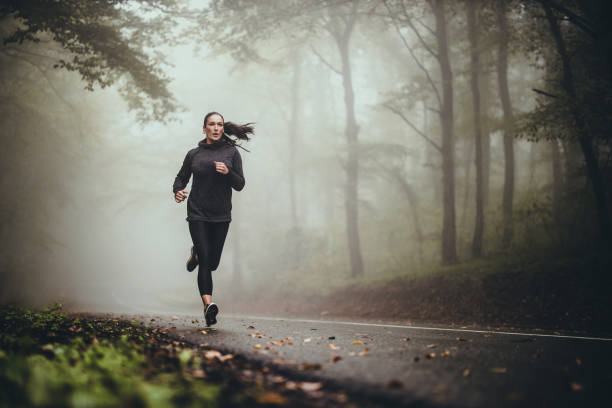
\includegraphics[trim=30 0 60 10,clip,width=\linewidth]{Ressources/2GT_C8_Exercices_Fig3.jpg}
\end{multicols}
\section{Connaître les caractéristiques du vecteur vitesse}
Les positions successives occupées par un système à intervalles de temps réguliers sont représentées ci-dessous.\\
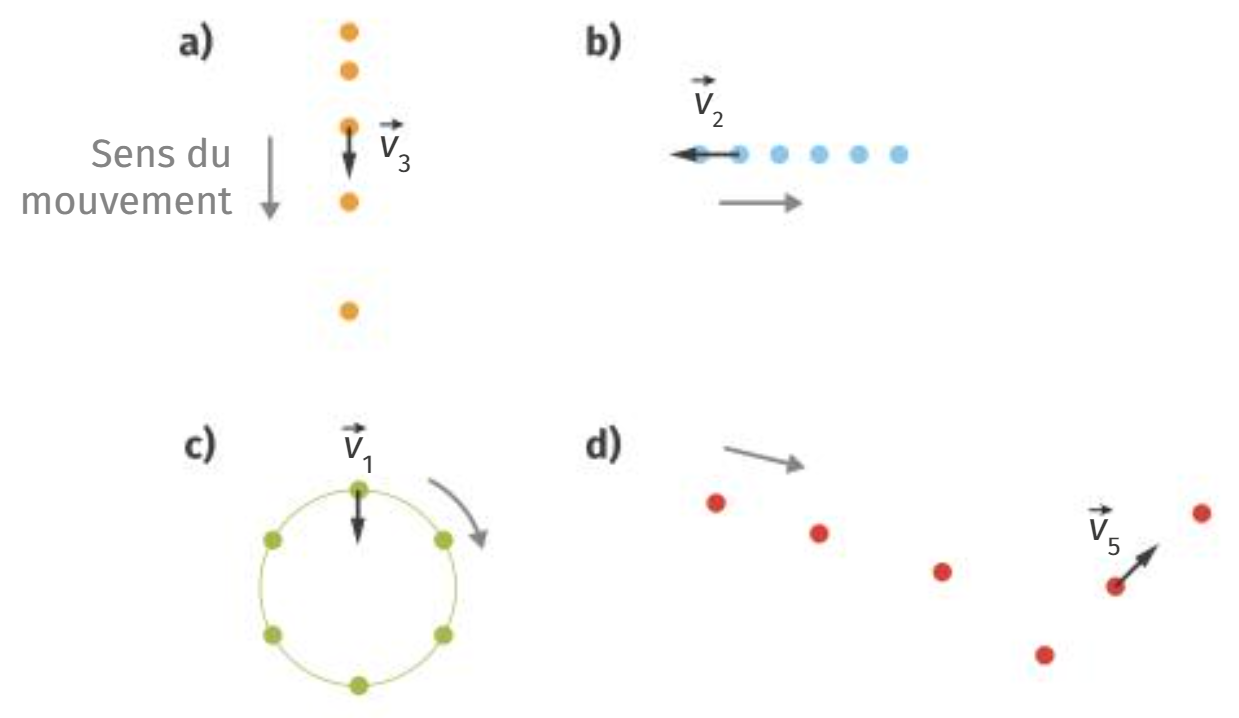
\includegraphics[width=\linewidth]{Ressources/2GT_C8_Exercices_Fig1.png}
\begin{enumerate}
	\item Décrire dans chacun des cas le mouvement du système en termes de trajectoire de variation de la vitesse.
	\item Parmi les vecteurs vitesse, lesquels sont correctement représentés ?
	\item Pour chacun des vecteurs vitesse erronés, expliquer l'erreur.
\end{enumerate}

\section{Astrophotographie}
\noindent 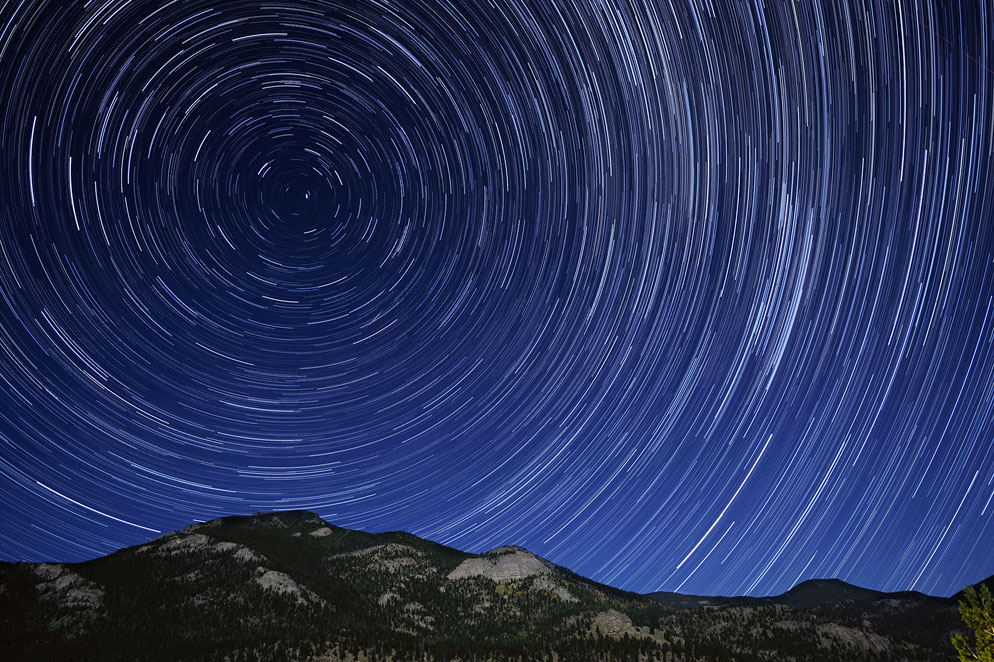
\includegraphics[width=\linewidth]{Ressources/2GT_C8_Exercices_Fig2.jpg}
\begin{enumerate}
	\item  Dans quel référentiel les étoiles sont-elles photographiées ?
	\item Décrire leur trajectoire.
	\item L'étoile polaire est une étoile qui paraît fixe par rapport à la Terre. Identifier cette étoile sur la photographie.
	\item En quoi le mouvement apparent des étoiles peut-il être un inconvénient en astrophotographie ?
	\item  Les astrophotographes professionnels sont équipés de télescopes motorisés qui suivent le mouvement d'une étoile. Expliquer pourquoi.
\end{enumerate}

\section{Station spatiale internationale}
La station spatiale internationale (ISS) est une station spatiale en orbite circulaire basse autour de la Terre. Des astronautes internationaux y mènent des expériences de recherche scientifique en milieu spatial. Située à une altitude d'environ 330 km, l'ISS effectue un tour complet en 93 minutes.
\begin{enumerate}
	\item Quel est le référentiel adapté à l’étude du mouvement de l’ISS ?
	\item Décrire le mouvement de l’ISS dans ce référentiel.
	\item Calculer la valeur de la vitesse de la station.
	\item Décrire la variation de son vecteur vitesse.
	\item Combien de tours effectue l’ISS en une journée ?
\end{enumerate}

\textbf{Donnée :} Rayon de la Terre $R_T$ = \SI{6370}{km}

\section{La grêle}
La grêle peut avoir des effets dévastateurs pour les habitants et les agriculteurs en raison de la vitesse que les grêlons acquièrent lors de leur chute. En effet, le grêlon chute avec une vitesse initiale nulle puis accélère jusqu'à atteindre une vitesse limite de \SI{70}{\kilo\meter\per\hour}.
\begin{enumerate}
	\item Définir le système et le référentiel d'étude.
	\item Le système est assimilé à un point matériel. Quel(s) aspect(s) ne peut-on pas aborder lors de cette étude ?
	\item Comment évolue le vecteur vitesse lors de la première phase de la chute ?
	\item Donner la direction, le sens et la norme du vecteur en \unit{\meter\per\second} lors de la deuxième phase de la chute.
	\item Comment qualifier le mouvement durant cette deuxième phase ?
\end{enumerate}
\end{multicols}
\end{document}